\documentclass{beamer}

\usepackage[utf8]{inputenc}
\usepackage[english]{babel}
\usepackage[T1]{fontenc}
\usepackage{lmodern}
\usepackage{adjustbox}
\usepackage{graphicx}
\usepackage{caption}
\usepackage{subcaption}
\usepackage{color, colortbl}
\usepackage{commath}
\usepackage{amsmath,amssymb,amsthm}
\usepackage{tikz}
\usepackage{pgffor}
\usepackage{enumitem}
\DeclareMathOperator*{\argmax}{arg\,max}
\DeclareMathOperator*{\argmin}{arg\,min}
\usepackage[lined]{algorithm2e}
\usetheme{Singapore}
\newlength{\mylen}
\resetcounteronoverlays{compt}
\addtobeamertemplate{navigation symbols}{}{%
    \usebeamerfont{footline}%
    \usebeamercolor[fg]{footline}%
    \hspace{1em}%
    \insertframenumber/\inserttotalframenumber
}
\usepackage{upgreek}
\usepackage[doi=false,
            isbn=false,
            url=false,
            bibstyle=authoryear,
            style=authoryear]{biblatex}
\bibliography{biblio}%
\renewcommand{\footfullcite}[1]{\footnote[frame]{\fullcite{#1}}}
\def\bibfont{\tiny}%
\begin{document}

\AtBeginSection[]{
  \begin{frame}{Outline}
  \small \tableofcontents[currentsection, hideothersubsections]
  \end{frame} 
}

\title{Viterbi Algorithm for Intrusion Type Identification in Anomaly
  Detection System}
\author{ } 
\institute{ }
\date{january 14th 2019}

\maketitle

\section{Introduction}

\begin{frame}
\frametitle{Context}
      \begin{figure}
        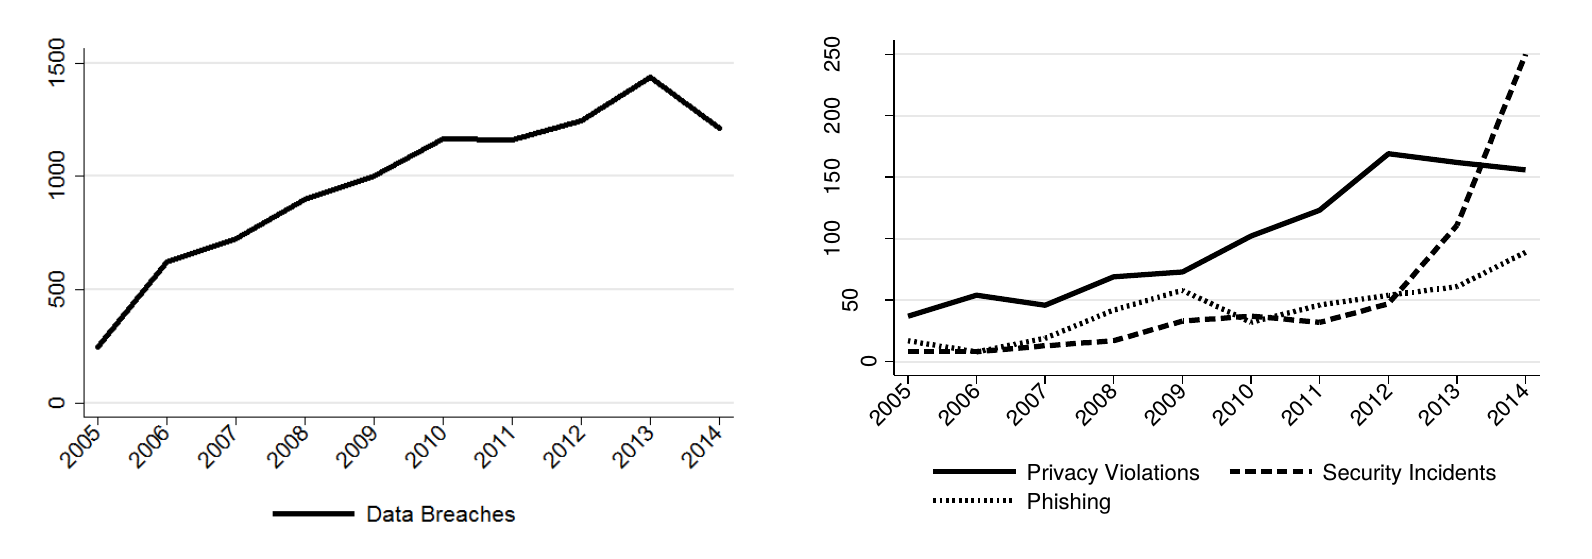
\includegraphics[scale=0.2]{img/increasintrusion.png}
         \footfullcite{romanosky2016examining}
       \end{figure}
       
  \begin{itemize}[label=.]
    \item Number of intrusions is increasing with time and can cause a lot of damage \pause
    \item In 2005, among 7,818 businesses 
    
    \begin{itemize}[label=.]
        \item Nearly 60\% detected one or more types of cyber attack. \textit{(National Computer Security Survey (NCSS))}
        \item Approximately 68\% of the victims of cyber theft sustained monetary loss of \$10,000 or more.
     \end{itemize}
  \end{itemize}
\end{frame}

\begin{frame}
  \frametitle{Intrusion Type}
  \begin{itemize}[label=.]
  \item Buffer overflow
    \begin{itemize}[label=.]
    \item xlock vulnerability
    \item lpset vulnerability
    \item kcms\_sparc vulnerability
    \end{itemize}
  \item S/W security vulnerability
  \item Setup vulnerability
  \item Denial of service
  \end{itemize}
\end{frame}

\begin{frame}{Intrusion Detection Systems (IDS)}
  \begin{itemize}[label=.]
        \item \textbf{host-based}:  related to OS information 
        \item \textbf{network based}:  network related events
  \end{itemize}
  \hspace{1cm}
  \begin{itemize}[label=.]
        \item \textbf{misuse-based}:  seek defined patterns, or signatures, within the analyzed data
        \item \textbf{anomaly-based}:  estimate the ‘‘normal’’ behaviour of the system to be protected, and generate an anomaly alarm whenever the deviation between a given observation at an instant and the normal behaviour exceeds a predefined threshold
\end{itemize}
\end{frame}

\begin{frame}{Intrusion Detection Systems (IDS)}
  \begin{itemize}[label=.]
        \item \textbf{\textcolor{red}{host-based}}:  related to OS information 
        \item \textbf{network based}:  network related events
  \end{itemize}
  \hspace{1cm}
  \begin{itemize}[label=.]
        \item \textbf{misuse-based}:  seek defined patterns, or signatures, within the analyzed data
        \item \textbf{\textcolor{red}{anomaly-based}}:  estimate the ‘‘normal’’ behaviour of the system to be protected, and generate an anomaly alarm whenever the deviation between a given observation at an instant and the normal behaviour exceeds a predefined threshold
\end{itemize}
\end{frame}

\section{Backgroung}
\begin{frame}
  \frametitle{Markov Chain}
  \begin{columns}[T]
    \begin{column}{.7\textwidth}
      A markov Chain \footfullcite{MarkovChain} is defined by :
      \begin{itemize}[label=.]
      \item S, A finite set of N states
      \item $\pi$, A vector of initial probabilities over S :
        $$\pi_i = P(S_1 = i), 1 \leq i \leq N$$
      \item A, A matrix of probabilities of transitions over $SxS$ :
        $$a_{ij} = P(S_t = j | S_{t-1} = i), 1 \leq i \leq N$$
      \item Markov assumption :
        $P(S_t|S_{t-1},S_{t-2},\ldots,S_{1})=P(S_t|S_{t-1})$ 
      \end{itemize}
    \end{column}
    \begin{column}{.28\textwidth}
      \begin{figure}
        \includegraphics[scale=0.4]{img/markov_chain_example.png}
        $$
        A = \begin{pmatrix}
          0.6 & 0.4 \\
          0.9 & 0.1
        \end{pmatrix}
        $$
        \caption{Simple example of Markov Chain}
      \end{figure}
    \end{column}
  \end{columns}
\end{frame}

\begin{frame}
  \frametitle{HMM - Hidden Markov Model}
  \begin{itemize}[label=--]
  \item Hidden Markov Model \footfullcite{baum1966statistical} is a statistical model in which the
    modeled system is supposed to be a Markovian process of unknown
    parameters.\pause
  \item Hidden Markov Model can be viewed as a Bayesian Network\pause
  \item We define a HMM including :
    \begin{itemize}
    \item V, A finite set of M observations
    \item B, A a matrix of probabilities of observations
      over state :
      $$b_i(k) = P(0_t=V_k | S_t = i)$$
    \end{itemize}
  \end{itemize}
\end{frame}

\begin{frame}
  \frametitle{HMM - Forward Algorithm}
  \scalebox{0.7}{
    \begin{algorithm}[H]
      \SetKwInOut{Input}{input }
      \SetKwInOut{Output}{output }
      \Input{$\lambda$ The model, $O$ Observed sequence}
      \Output{ $P(0|\lambda)$}
      Step 1, Initialization :
        $
        \forall i, \alpha_1(i) = \pi_i b_i(O_1)
        $\\
        Step 2, Induction :\\
        \For{$t\gets2:T$}{
          $
          \forall i, \alpha_t(i) = \left[ \sum\limits_{j=1}^N\alpha_{t-1}(i)a_{ij}\right]
          b_j(O_t)
          $
        }
        Step 3, Termination :
        $
        P(0|\lambda) = \sum\limits_{i=1}^N \alpha_T(i)
        $
    \end{algorithm}
  }
  \footfullcite{forward_algo}
\end{frame}

\begin{frame}
  \frametitle{HMM - Viterbi Algorithm}
  \scalebox{0.6}{
    \begin{algorithm}[H]
      \SetKwInOut{Input}{input }
      \SetKwInOut{Output}{output }
      \Input{$O$ Observed sequence}
      \Output{ $\argmax\limits_{\lambda \in \Lambda} P(0|\lambda)$}
      Step 1, Initialization :\\
      \For{$i\gets1:N$}{
        $\delta_1(i) = \pi_i b_i(0_1)$\\
        $\psi_1(i) = 0$
      }
      Step 2, Recursion :\\
      \For{$t\gets2:T$}{
        \For{$j\gets1:N$}{
          $\delta_t(j) = \max\limits_i [\delta_{t-1}(i)a_{ij}]b_j(0_t)$\\
          $\psi_t(j) = \argmax\limits_i [\delta_{t-1}(i)a_{ij}]b_j(0_t)$
        }
      }
      Step 3, Termination :\\
      $P^{*} = \max\limits_{s \in S}[\delta_T(s)]$\\
      $S_T^{*} = \argmax\limits_{s \in S}[\delta_T(s)]$\\
      Step 4, Backtracking :\\ 
      \For{$t\gets{T-1}:1$}{
        $S_t^{*} = \psi_{t+1}(s_{t+1 }^{*})$
      }
      \Return{$S^{*}$}
    \end{algorithm}
        }
        \footfullcite{viterbi}
\end{frame}
\section{Proposed Method}
\subsection{Intrusion Detection}
\begin{frame}
  \frametitle{Normal Behaviour Modeling}
  \begin{itemize}
  \item Normal Behaviour is modelised by a left-to-right HMM $\lambda$.
    \begin{figure}
      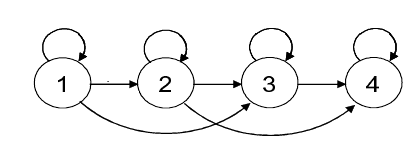
\includegraphics[scale=0.4]{img/left_to_right.png} 
      \caption{Left-to-Right Model with jumps}
    \end{figure}
  \item The forward allgorithm is used to decide whether normal or not
    with a threshold.
  \end{itemize}
\end{frame}
\begin{frame}
  \frametitle{Intrusion Detection}
  \framesubtitle{Data}
  $S = \{1,2,3,4\}$\\
  $M = \{1,2,3,4\}$\\
  $\pi = \{1.0,0,0\}$\\
  $O = \{2,1,2,4,2,3,4,3,4,3\}$
  \begin{columns}[T]
    \begin{column}{.45\textwidth}
      $$
      A = \begin{pmatrix}
        0.28 & 0.34 & 0.28 & 0\\
        0.0 & 0.32 & 0.21 & 0.47\\
        0.0 & 0.0 & 0.32 & 0.68\\
        0.0 & 0.0 & 0.0 & 1.0
      \end{pmatrix}
      $$
    \end{column}
    \begin{column}{.45\textwidth}
      $$
      B = \begin{pmatrix}
        0.8 & 0.04 & 0.1 & 0.06\\
        0.0 & 0.13 & 0.45 & 0.42\\
        0.0 & 0.9 & 0.1 & 0.0\\
        0.64 & 0.12 & 0.06 & 0.18\\
      \end{pmatrix}
      $$
    \end{column}
  \end{columns}
\end{frame}

\begin{frame}
  \frametitle{Intrusion Detection}
  \framesubtitle{initialization}
  \scalebox{1}{
    \begin{algorithm}[H]
      $
      \forall i, \alpha_1(i) = \pi_i b_i(O_1)
      $\\
    \end{algorithm}
  }\pause
\\  $\pi = \{1.0,0,0\}$\\
  $O = \{\textcolor{red}{2},1,2,4,2,3,4,3,4,3\}$
  \begin{columns}[T]
    \begin{column}{.45\textwidth}
      $$
      A = \begin{pmatrix}
        0.28 & 0.34 & 0.28 & 0\\
        0.0 & 0.32 & 0.21 & 0.47\\
        0.0 & 0.0 & 0.32 & 0.68\\
        0.0 & 0.0 & 0.0 & 1.0
      \end{pmatrix}
      $$
    \end{column}
    \begin{column}{.45\textwidth}
      $$
      B = \begin{pmatrix}
        0.8 & \textcolor{red}{0.04} & 0.1 & 0.06\\
        0.0 & \textcolor{red}{0.13} & 0.45 & 0.42\\
        0.0 & \textcolor{red}{0.9} & 0.1 & 0.0\\
        0.64 & \textcolor{red}{0.12} & 0.06 & 0.18\\
      \end{pmatrix}
      $$
    \end{column}
  \end{columns}
\end{frame}


\begin{frame}
  \frametitle{Intrusion Detection}
  \framesubtitle{Initialization}
  \scalebox{1}{
    \begin{algorithm}[H]
      $
      \forall i, \alpha_1(i) = \pi_i b_i(O_1)
      $\\
    \end{algorithm}
  }
  $$
  \begin{array}{ll}
    O_1 =& 2 \\
    b_i(O_1) =& (0.04, 0.13, 0.9, 0.12)\\ \pause
    \alpha_1(1) =& \pi_1 * b_1(O_1) = 1 * 0.04 = 0.04 \\ \pause
    \alpha_1(2) =& \pi_2 * b_2(O_1) =0 * 0.13 = 0 \\ \pause
    \ldots \\
    \alpha_1 =& \begin{pmatrix} 0.04 & 0 & 0 & 0\end{pmatrix}
  \end{array}
  $$
\end{frame}
\begin{frame}
  \frametitle{Intrusion Detection}
  \framesubtitle{Induction}
  \scalebox{0.8}{
    \begin{algorithm}[H]
      \For{$t\gets2:T$}{
        $
        \forall i, \alpha_t(i) = \left[ \sum\limits_{j=1}^N\alpha_{t-1}(i)a_{ij}\right]
        b_j(O_t)
        $
      }
    \end{algorithm}
  }
  \pause
  $$
  \begin{array}{ll}
    t= & 2\\
    O_2 =& 1 \\
    b(O_t) =& \begin{pmatrix}0.8& 0& 0& 0.64\end{pmatrix}\\
    \alpha_1 =& \begin{pmatrix} 0.04 & 0 & 0 & 0\end{pmatrix}\\ \pause
    \alpha_2(1) =& \left[ \sum\limits_{j=1}^N\alpha_{t-1}(1)a_{1j}\right] b_j
                   (O_t) = 0.00896 \\ \pause
       & \ldots \\
    \alpha_2 =& \begin{pmatrix} 0.00896 & 0 & 0 & 0\end{pmatrix}\\
  
  \end{array}
  $$
\end{frame}
\begin{frame}
  \frametitle{Intrusion Detection}
  \framesubtitle{Induction}
  \scalebox{0.8}{
    \begin{algorithm}[H]
      \For{$t\gets2:T$}{
        $
        \forall i, \alpha_t(i) = \left[ \sum\limits_{j=1}^N\alpha_{t-1}(i)a_{ij}\right]
        b_j(O_t)
        $
      }
    \end{algorithm}
  }
  $$
  \alpha = 
  \begin{pmatrix} 
    0.04 & 0 & 0 & 0\\
    0.00896 & 0 & 0 & 0\\
    0.00010035 & 0.00039603 & 0.0022579 & 0\\
    1.8882e^{-08} & 2.8849e^{-06} & 1.3193e^{-05} & 4.0995e^{-05}\\
    1.6859e^{-06} & 5.3227e^{-05} & 0& 0.00027637\\
    5.287e^{-10} & 4.1831e^{-07} & 4.8329e^{-07} & 3.0793e^{-06}\\
    8.8822e^{-12} & 5.6297e^{-08}& 0 & 6.4882e^{-07} \\
    2.487e^{-13} & 8.1081e^{-09} & 1.1825e^{-09} & 4.0517e^{-08}\\
    4.1782e^{-15} & 1.0898e^{-09} & 0& 8.1237e^{-09}\\
    1.1699e^{-16} & 1.5693e^{-10} & 2.2885e^{-11} & 5.1816e^{-10}
  \end{pmatrix}
  $$
\end{frame}
\begin{frame}
  \frametitle{Intrusion Detection}
  \framesubtitle{Termination}
  $$
  \begin{array}{ll}
    P(0|\lambda)) = &\sum\limits_{i=1}^N \alpha_T(i) \\
                   & = 1.1699e^{-16} + 1.5693e^{-10} + 2.2885e^{-11} + 5.1816e^{-10} \\
                   &= 6.9797e^{-10}
  \end{array}
$$
\end{frame}
\begin{frame}
  \frametitle{Intrusion Detection}
  \framesubtitle{Decision}
  \scalebox{0.7}{
    \begin{algorithm}[H]
      \uIf{$log(P(0|\lambda)) >~threshold$}{
        \Return{Normal Behaviour} 
      }
      \Else{
        \Return{Intrusion}
      }
    \end{algorithm}
    }
  $$
  log(P(0|\lambda) = -21.083 < threshold (-20.83) \implies Intrusion
  $$
\end{frame}
\begin{frame}
  \frametitle{Intrusion Detection}
  \framesubtitle{Results}
  \begin{table}[h]
    \centering
    \caption{\label{tab:IDS}The performance of HMM-based IDS. Best
      results are in bold}
    \begin{tabular}{|c |c | c | c |}
      \hline
      Length & Thresold & Detection Rate & F-P Error \\ \hline
      10 & -9.43 & 100\% & 2.626 \\ \hline
      15 & -9.43 & 100\% & 3.614 \\ \hline
      10 & -14.42 & 100\% & 1.366 \\ \hline
      15 & -14.42 & 100\% & 2.718 \\ \hline
      10 & -16.94 & 100\% & 0.789 \\ \hline
      15 & -16.94 & 100\% & 2.618 \\ \hline
      10 & -18.35 & 100\% & 0.553 \\ \hline
      15 & -18.35 & 100\% & 2.535 \\ \hline
      10 & -19.63 & 100\% & 0.476 \\ \hline
      15 & -19.63 & 100\% & 2.508 \\ \hline
      \textbf{10} & \textbf{-20.83} & \textbf{100\%} & \textbf{0.372}
      \\ \hline
      15 & -20.83 & 100\% & 2.473 \\ \hline
    \end{tabular}
  \end{table}    
\end{frame}
\subsection{Intrusion Type Identification}
\begin{frame}
  \frametitle{Intrusion Type Identification}
  Process in two steps :
  \begin{itemize}
  \item Viterbi algorithm is used to find the optimal state sequence
  \item Euclidean distance is used to identify the intrusion type with the
    optimal state sequence
  \end{itemize}
\end{frame}
\begin{frame}
  \frametitle{Intrusion Type Identification}
  \framesubtitle{Data}
  $S = \{1,2,3,4\}$\\
  $M = \{1,2,3,4\}$\\
  $\pi = \{1.0,0,0\}$\\
  $O = \{2,1,2,4,2,3,4,3,4,3\}$
  \begin{columns}[T]
    \begin{column}{.45\textwidth}
      $$
      A = \begin{pmatrix}
        0.28 & 0.34 & 0.28 & 0\\
        0.0 & 0.32 & 0.21 & 0.47\\
        0.0 & 0.0 & 0.32 & 0.68\\
        0.0 & 0.0 & 0.0 & 1.0
      \end{pmatrix}
      $$
    \end{column}
    \begin{column}{.45\textwidth}
      $$
      B = \begin{pmatrix}
        0.8 & 0.04 & 0.1 & 0.06\\
        0.0 & 0.13 & 0.45 & 0.42\\
        0.0 & 0.9 & 0.1 & 0.0\\
        0.64 & 0.12 & 0.06 & 0.18\\
      \end{pmatrix}
      $$
    \end{column}
  \end{columns}
\end{frame}
\begin{frame}
  \frametitle{Intrusion Type Identification}
  \framesubtitle{Initialization}
  \scalebox{1}{
    \begin{algorithm}[H]
      \For{$i\gets1:N$}{
        $\delta_1(i) = \pi_i b_i(0_1)$\\
        $\psi_1(i) = 0$
      }
    \end{algorithm}
  }
  $$
  \begin{array}{ll}
    O_1 =& 2 \\
    b_i(0_1) =& (0.04, 0.13, 0.9, 0.12)\\ \pause
    \delta_1(1) =& \pi_1 * b_1(0_1) = 1 * 0.04 = 0.04 \\ \pause
    \delta_1(2) =& \pi_2 * b_2(0_1) =0 * 0.13 = 0 \\ \pause
    \ldots \\
    \delta_1 = \begin{pmatrix} 0.04 & 0 & 0 & 0\end{pmatrix}
  \end{array}\pause
  $$
  $$
  \psi_1 = \begin{pmatrix}0&0&0&0\end{pmatrix}
  $$
\end{frame}
\begin{frame}
  \frametitle{Intrusion Type Identification}
  \framesubtitle{Recursion}
  \scalebox{0.6}{
    \begin{algorithm}[H]
      \For{$t\gets2:T$}{
        \For{$j\gets1:N$}{
          $\delta_t(j) = \max\limits_i [\delta_{t-1}(i)a_{ij}]b_j(0_t)$\\
          $\psi_t(j) = \argmax\limits_i [\delta_{t-1}(i)a_{ij}]b_j(0_t)$
        }
      }
    \end{algorithm}
  }
\begin{equation*}
  \begin{array}{ll}
    t = & 2 \\
    O_2 =& 1 \\
    \delta_1 = & \begin{pmatrix} 0.04 & 0 & 0 & 0\end{pmatrix}\\ \pause
    \delta_2(1) = & \max\limits_i [\delta_{t-1}(i)a_{i1}]b_1(0_2) \\
    = & 0.00896 \\
    \delta_2 = & \begin{pmatrix} 0.00896 &0 & 0& 0\end{pmatrix}\\ \pause
    \psi_2(1) = & \argmax\limits_i [\delta_{t-1}(i)a_{i1}]b_1(0_2) \\
    = & 0 \\  \pause
    \psi_2 = & \begin{pmatrix} 0 &0 & 0& 0\end{pmatrix}
  \end{array}
\end{equation*}
 \end{frame}
\begin{frame}
  \frametitle{Intrusion Type Identification}
  \framesubtitle{Recursion}
  \scalebox{0.6}{
    \begin{algorithm}[H]
      \For{$t\gets2:T$}{
        \For{$j\gets1:N$}{
          $\delta_t(j) = \max\limits_i [\delta_{t-1}(i)a_{ij}]b_j(0_t)$\\
          $\psi_t(j) = \argmax\limits_i [\delta_{t-1}(i)a_{ij}]b_j(0_t)$
        }
      }
    \end{algorithm}
  }
  \begin{columns}[T]
    \begin{column}{.73\textwidth}
      \begin{equation*}
        \resizebox{\textwidth}{!}{$
          \delta = 
          \begin{pmatrix}
            0.04 & 0& 0& 0\\
            0.00896&0&0&0\\
            0.00010035&0.00039603&0.0022579&0\\
            1.6859e^{-06}&5.3227e^{-05}&0&0.00027637\\
            1.8882e^{-08}&2.2142e^{-06}&1.006e^{-05}&3.3164e^{-05}\\
            5.287e^{-10}&3.1885e^{-07}&3.2192e^{-07}&1.9899e^{-06}\\
            8.8822e^{-12}&4.2853e^{-08}&0&3.5817e^{-07}\\
            2.487e^{-13}&6.1709e^{-09}&8.9992e^{-10}&2.149e^{-08}\\
            4.1782e^{-15}&8.2937e^{-10}&0&3.8683e^{-09}\\
            1.1699e^{-16}&1.1943e^{-10}&1.7417e^{-11}&2.321e^{-10}
          \end{pmatrix}
          $}
      \end{equation*}
    \end{column}
    \begin{column}{.23\textwidth}
      \begin{equation*}
        \resizebox{\textwidth}{!}{$
          \psi = 
          \begin{pmatrix}
            0&0&0&0\\
            0&0&0&0\\
            0&0&0&0\\
            0&1&0&2\\
            0&1&1&3\\
            0&1&2&3\\
            0&1&0&3\\
            0&1&1&3\\
            0&1&0&3\\
            0&1&1&3
          \end{pmatrix}
          $}
      \end{equation*}
    \end{column}
  \end{columns}
  \end{frame}
\begin{frame}
  \frametitle{Intrusion Type Identification}
  \framesubtitle{Termination}
  $$
  P^{*} = \max\limits_{s \in S}[\delta_T(s)] = 2.321e^{-10}
  $$
\end{frame}
\begin{frame}
  \frametitle{Intrusion Type Identification}
  \framesubtitle{Backtracking}
  \scalebox{0.6}{
    \begin{algorithm}[H]
      \For{$t\gets{T-1}:1$}{
        $S_t^{*} = \psi_{t+1}(s_{t+1 }^{*})$
      }\end{algorithm}
  }\\
  Optimal Sequence $ S^{*} = \{1,1,3,4,4,4,4,4,4,4\}$
\end{frame}
\begin{frame}
  \frametitle{Intrusion Type Identification}
  \framesubtitle{Decision}
  \begin{table}
    \caption{\label{tab:type}Sequences for each type of intrusion}
    \begin{tabular}{|c|c|c|}
      \hline
      Type & Sequence & Distance \\ \hline
      xlock & $\{2,2,3,3,3,4,4,4,4,4\}$ & $3.7417$ \\ \hline
      ipset & $\{2,3,3,3,4,4,4,4,4,4\}$ & $4.4721$ \\ \hline
      kcms\_sparc & $\{1,1,2,2,2,2,4,4,4,4\}$ & $3$ \\ \hline
    \end{tabular}
  \end{table}
\end{frame}
\begin{frame}
  \frametitle{Intrusion Type Identification}
  \framesubtitle{Results}
  \begin{table}[h]
    \centering
    \caption{\label{tab:IDS}The performance of Viterbi-based Intrusion
      Type Identification. (A:xlock, B: lpset, C:
kcms\_sparc, D: processe creation, E: fill the disk, F: exhausting the memory)}
    \begin{tabular}{|c| c|c | c | c | c | c | c |}
      \hline & A & B &C &D &E &F &Rate \\ \hline
      A & 8 & 1 & \_ & \_ & \_ & \_ & $88\%$ \\ \hline
      B & \_ & 6 & 1  & \_ & \_ & \_& $86\%$ \\ \hline
      C & \_ & \_ & 4 & \_ & \_ & \_ & $100\%$ \\ \hline
      D & \_ & \_ & \_ & 3 & \_ & 6 &$33\%$ \\ \hline \hline
      E & \_ & \_ & \_ & 4 & \_ & 3 &$0\%$ \\ \hline
      F & \_ & \_ & \_ & 2 & 1 & 6 &$66\%$ \\ \hline
    \end{tabular}
  \end{table}    
\end{frame}
\begin{frame}
  \frametitle{Intrusion Type Identification}
  \framesubtitle{Results}
  \begin{table}[h]
    \centering
    \caption{\label{tab:IDS}The performance of Viterbi-based Intrusion
      Type Identification}
    \begin{tabular}{|c| c|c | c | c |}
      \hline
      Attack & Trial & Correct & Incorrect & Rate \\ \hline
      Buffer Overflow & 20 & 18 & 2 & 90\% \\ \hline
      Denial of Service & 25 & 9 & 16 & 36\% \\ \hline
      All  & 45 & 27 & 18 & 60\% \\ \hline
    \end{tabular}
  \end{table}    
\end{frame}

\section{Limitations \& Remarks}
\begin{frame}
  \frametitle{Limitations \& Remarks}
  \begin{itemize}[label=$\square$]
  \item Try other distance metrics for Intrusion Type Identification :
    \fullcite{10.1007/11590316_30}\pause
  \item Hypothesis that there is only one sequence of state per each intrusion, 
    and that it never changes.\pause
  \item This model is anomaly-based, but use the fact that we are supposed to 
    know the sequence of state of the intrusion. they loose the main advantage 
    of anomaly-based IDS to detect new types of intrusion.
  \end{itemize}
\end{frame}

\begin{frame}
  \frametitle{Limitations \& Remarks}
  \begin{itemize}[label=$\square$]
  \item  Low detection efficiency, especially due to the high false positive 
    rate usually obtained \fullcite{axelsson1998research}\pause
  \item Absence of appropriate metrics and assessment methodologies, as well as 
    a general framework for evaluating and comparing alternative IDS techniques
    \fullcite{stolfo2000cost}
  \end{itemize}
\end{frame}

\section{Other Method}
\begin{frame}
  \frametitle{Methods using HMM}
  \framesubtitle{Intrusion Alert Prediction Using a Hidden Markov Mode}
  \begin{itemize}
  \item Alert prediction method  based on prediction of the next alert cluster
  \item Clusters  contains :
    \begin{itemize}[label=-]
    \item source IP address
    \item destination IP range
    \item alert type
    \item alert category.
    \end{itemize}
  \item Prediction of next alert cluster provides more information about future 
    strategies of the attacker and does not depend on specific domain knowledge
  \end{itemize}
  \footfullcite{thanthrige2016intrusion}
\end{frame}

\begin{frame}
  \frametitle{Methods using HMM}
  \framesubtitle{Anomalybased HMMs}
  \begin{itemize}
  \item Used for intrusion detection, with five states and six observation 
    symbols per state
  \item States in the model are interconnected in such a way that any state can
    be reached from any other state
  \item Baum-Welch method is used
  \end{itemize}
  \footfullcite{joshi2005investigating}
\end{frame}

\begin{frame}
  \frametitle{Other Methods}
  \begin{figure}
    \centering
    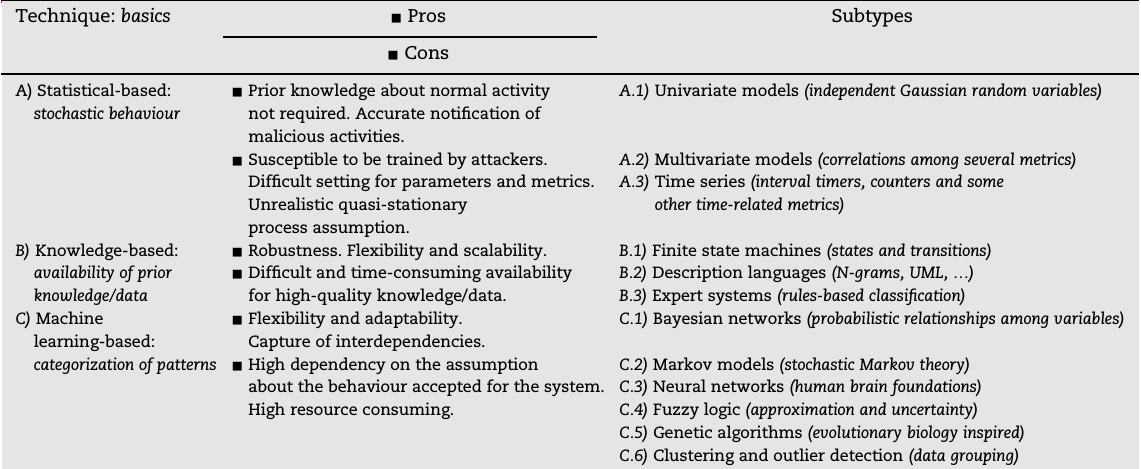
\includegraphics[scale=0.3]{img/modelComparison1.png} 
    \footfullcite{garcia2009anomaly}
  \end{figure}
\end{frame}

\begin{frame}
  \frametitle{Other Methods}
  \begin{figure}
    \centering
    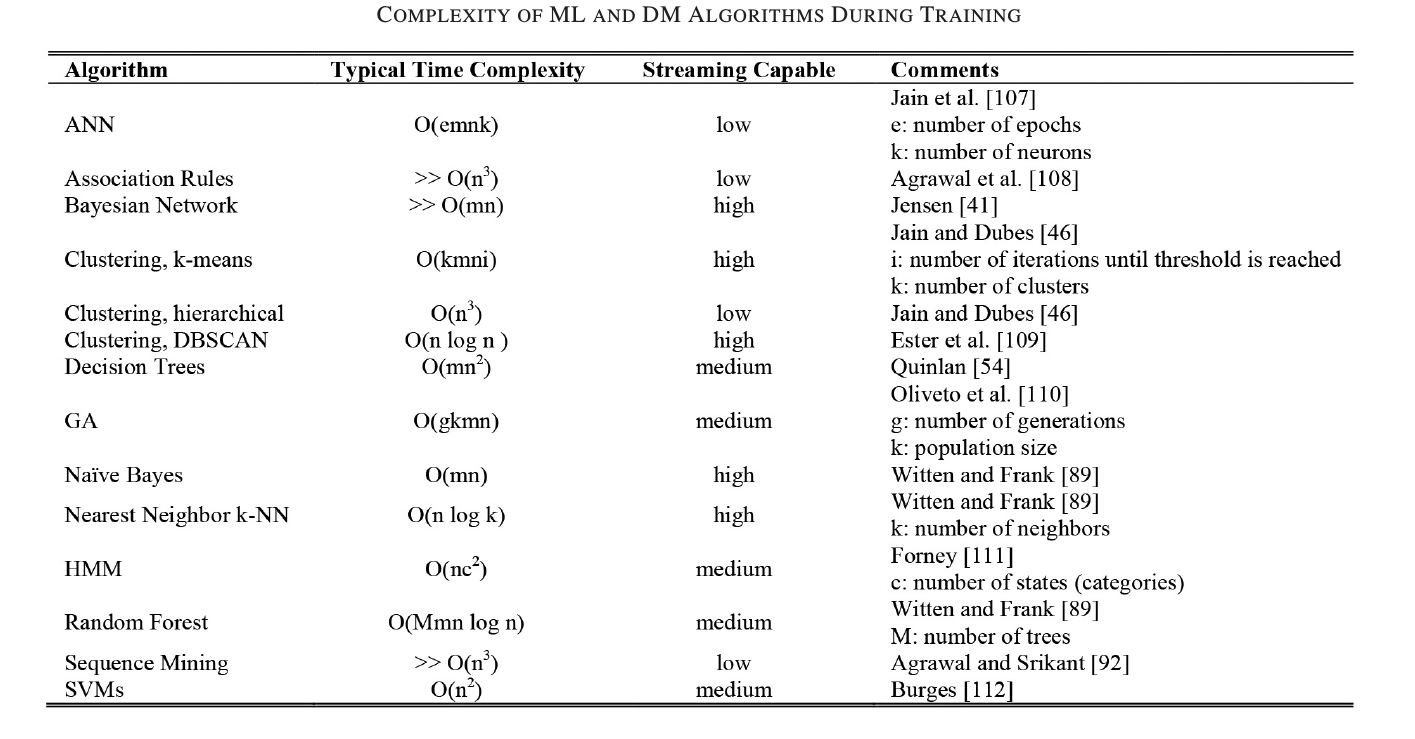
\includegraphics[scale=0.25]{img/modelComparison2.png}
    \footfullcite{buczak2016survey}
  \end{figure} 
\end{frame}

\section{Conclusion}
\begin{frame}
  \frametitle{Conclusion}
  \begin{itemize}
  \item Good results for Intrusion detection
  \item For type indentification :
    \begin{itemize}
    \item Good results for Buffer Overflow (90\%)
    \item Bad results for Denial of Service (36\%)
    \end{itemize}
  \end{itemize}
\end{frame}

\begin{frame}
Any question ?
\end{frame}
\end{document}
